
\item[(b)] In an experiment to determine hydrolysable tannins in plants by absorption spectroscopy, the following results from ten samples were obtained and are tabulated below. A simple linear regression model, predicting absorbance values using concentration as the independent variable, was fitted to the data. The scatterplot is depicted below.
%%Absorbance= c(0.084, 0.183, 0.326, 0.464, 0.643, 0.707, 0.717, 0.734 ,0.749 ,0.732) ;
%%Concentration= c(0.123, 0.288, 0.562, 0.921, 1.420, 1.717, 1.921, 2.137 ,2.321, 2.467) ;
%%plot(Concentration,Absorbance,pch=18,col="red",font.axis=2,font.lab=2)
%%abline(coef(lm(Absorbance~Concentration)))

%%Conc.Squared = (Concentration^2)
%%Conc.Cubed = (Concentration^3)
%%ModelA = lm(Absorbance~Concentration)
%%ModelB = lm(Absorbance~Concentration+Conc.Squared)
%%ModelC = lm(Absorbance~Concentration+Conc.Squared+Conc.Cubed)
\begin{center}
	\begin{tabular}{|c||c|c|c|c|c|}
		\hline
		%  % after \\: \hline or \cline{col1-col2} \cline{col3-col4} ...
		Sample & 1 & 2 & 3 & 4 & 5 \\ \hline
		Absorbance & 0.084& 0.183& 0.326& 0.464& 0.643\\
		Concentration & 0.123& 0.288& 0.562& 0.921& 1.420\\ \hline
		Sample & 6 & 7 & 8 & 9 & 10 \\ \hline
		Absorbance & 0.707& 0.717& 0.734 &0.749 &0.732\\
		Concentration & 1.717& 1.921& 2.137 &2.321&2.467\\
		\hline
	\end{tabular}
\end{center}
\begin{center}
	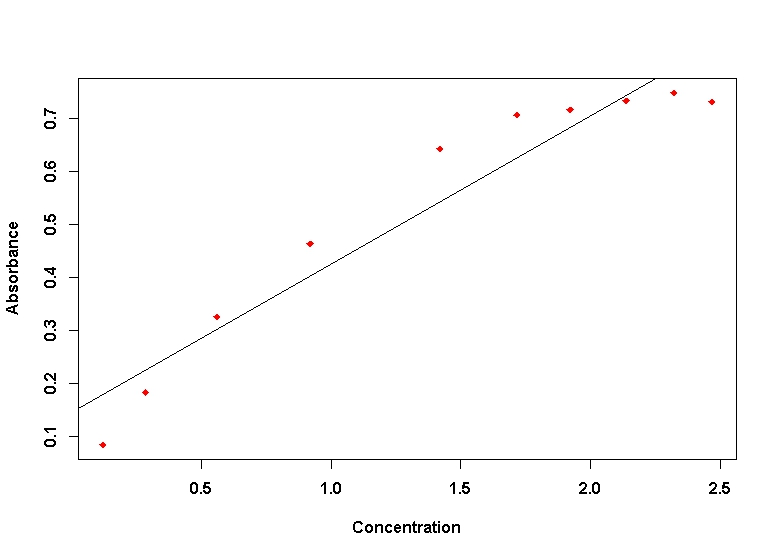
\includegraphics[scale=0.45]{images/ExamQ3plot}
\end{center}
\begin{itemize}
	\item[(i.)] (1 marks) Is the simple linear regression model approach suitable for this study? Explain your answer with reference to the scatter-plot.
	\item[(ii.)] (3 marks) Two polynomial models were also fitted to the data. Description of all three fitted models are found in the three blocks of \texttt{R} code on the following pages. The \emph{Akaike information criterion} is listed, for each of the three fitted models. Write down the regression equations of each of the three models.
	\item[(iii.)] (2 marks) Specify which one of the models you would use. Justify your answer with appropriate statistical values.
	\item[(iv.)] (2 marks) Using the best fitting model, predict a value for absorbance when the concentration level is 1.2 $mg/ml$.
	
\end{itemize}



%
%
%
%\item[(d)] Two polynomial models were also fitted to the data. Description of all three fitted models are found in the three blocks of \texttt{R} code below. The \emph{Akaike information criterion} is also listed, for each of the three fitted models.
%\begin{itemize}
%\item[i.] (4 marks) Write down the regression equation for each of the three linear models.
%\item[ii.] (2 marks) Based on the \emph{Akaike information criterion}, which fitted model can be assumed to be the best fit of the three candidate models.

%\end{itemize}
%\newpage


\begin{framed}
	\noindent \textbf{Model 1}
	\begin{verbatim}
	> summary(Model1)
	Call:
	lm(formula = Absorb ~ Conc)
	...
	Coefficients:
	Estimate Std. Error t value Pr(>|t|)
	(Intercept)    0.14412    0.04721   3.053   0.0158 *
	Concentration  0.28088    0.02930   9.586 1.16e-05 ***
	---
	Signif. codes:  0 ‘***’ 0.001 ‘**’ 0.01 ‘*’ 0.05 ‘.’ 0.1 ‘ ’ 1
	
	Residual standard error: 0.07584 on 8 degrees of freedom
	Multiple R-squared: 0.9199,     Adjusted R-squared: 0.9099
	F-statistic: 91.89 on 1 and 8 DF,  p-value: 1.163e-05
	>
	>
	>AIC(Model1)
	[1] -19.4343
	\end{verbatim}
\end{framed}

\begin{framed}
	\noindent	\textbf{Model 2}
	\begin{verbatim}
	> summary(Model2)
	Call:
	lm(formula = Absorb ~ Conc + Conc.Squared)
	...
	Coefficients:
	Estimate Std. Error t value Pr(>|t|)
	(Intercept)    0.006582   0.008013   0.821    0.439
	Concentration  0.642935   0.015568  41.299 1.27e-09 ***
	Conc.Squared  -0.140573   0.005894 -23.851 5.79e-08 ***
	---
	Signif. codes:  0 ‘***’ 0.001 ‘**’ 0.01 ‘*’ 0.05 ‘.’ 0.1 ‘ ’ 1
	
	Residual standard error: 0.008939 on 7 degrees of freedom
	Multiple R-squared: 0.999,      Adjusted R-squared: 0.9987
	F-statistic:  3592 on 2 and 7 DF,  p-value: 2.879e-11
	>
	>
	> AIC(Model2)
	[1] -61.5338
	\end{verbatim}
\end{framed}


\begin{framed}
	\noindent \textbf{Model 3}
	\begin{verbatim}
	> summary(Model3)
	
	Call:
	lm(formula = Absorb ~ Conc+ Conc.Squared + Conc.Cubed)
	...
	...
	Coefficients:
	Estimate Std. Error t value Pr(>|t|)
	(Intercept)    0.013712   0.011629   1.179   0.2830
	Concentration  0.608682   0.042825  14.213 7.58e-06 ***
	Conc.Squared  -0.108186   0.038088  -2.840   0.0296 *
	Conc.Cubed    -0.008196   0.009518  -0.861   0.4223
	---
	Signif. codes:  0 ‘***’ 0.001 ‘**’ 0.01 ‘*’ 0.05 ‘.’ 0.1 ‘ ’ 1
	
	Residual standard error: 0.009109 on 6 degrees of freedom
	Multiple R-squared: 0.9991,     Adjusted R-squared: 0.9987
	F-statistic:  2306 on 3 and 6 DF,  p-value: 1.422e-09
	>
	>
	> AIC(Model3)
	[1] -60.69903
	\end{verbatim}
\end{framed}
\newpage
%-------------------------------Start of Question 2B%
%\item[(b)](6 marks)
%The scatter-plot contains the regression line for the fitted model. Three diagnostic plots, used to assess the suitability of the fitted model, are presented on the following pages. Provide a brief interpretation for each of the three diagnostic plots described in part(a). The scatter-plot for the data is also presented.

%\begin{center}
%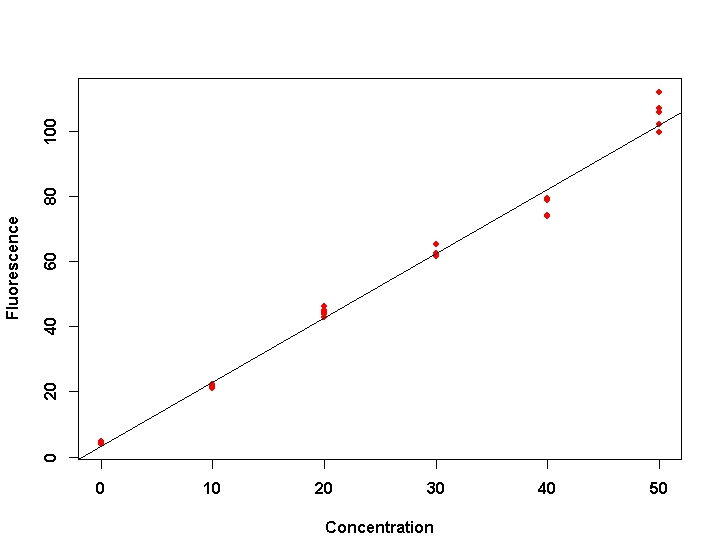
\includegraphics[scale=0.60]{ExamQ2plot2}
%\end{center}
%\newpage
%\begin{center}
%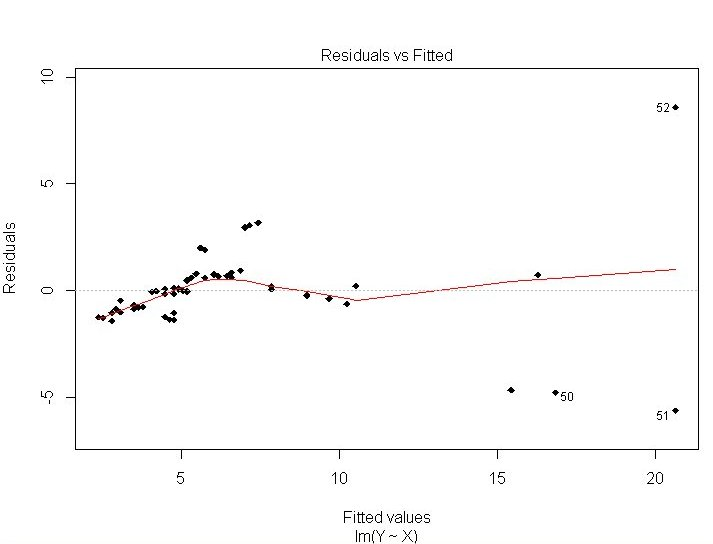
\includegraphics[scale=0.55]{ExamQ2diag1}
%\end{center}
%
%\begin{center}
%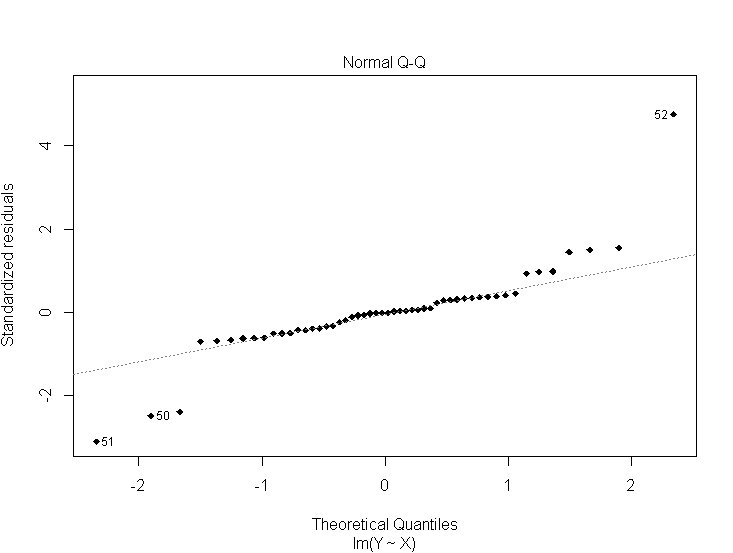
\includegraphics[scale=0.55]{ExamQ2diag2}
%\end{center}
%
%\begin{center}
%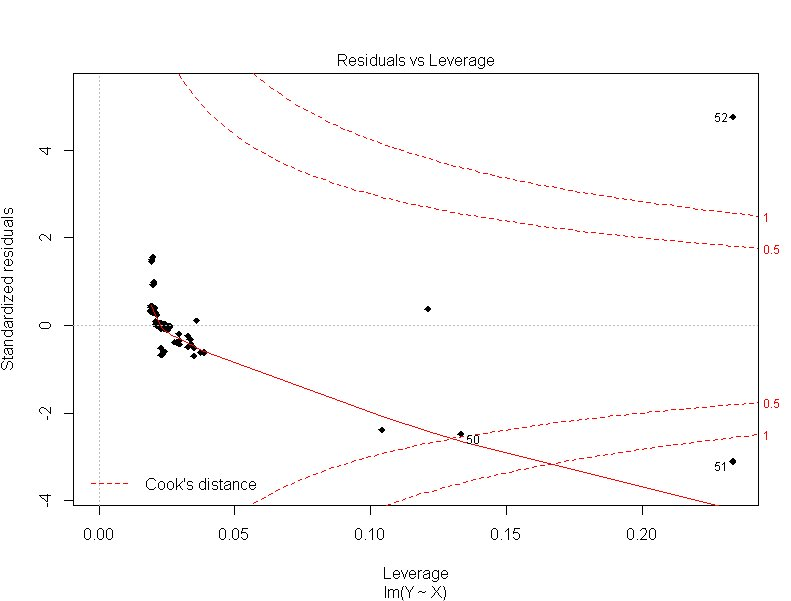
\includegraphics[scale=0.55]{ExamQ2diag3}
%\end{center}









\item[(e)]
The mercury level of several tests of sea-water from costal areas was determined by atomic-absorption spectrometry. The results obtained are as follows
\begin{center}
	\begin{tabular}{|c||c|c|c|c|c|c|c|c|c|c|c|} \hline
		Conc &0 &10&20&30&40&50&60&70&80&90&100 \\ \hline 
		Abso &0.321& 0.834& 1.254& 1.773& 2.237& 2.741& 3.196& 3.678& 
		4.217& 4.774& 5.261 \\ \hline
	\end{tabular} 
	
\end{center}



The analysis of the relationship between concentration and absorbance is obtained in R and presented below. 
\begin{framed}
	\begin{verbatim}
	x<-seq(0,100,by=10)
	y<- c(0.321, 0.834, 1.254, 1.773, 2.237, 2.741, 3.196, 3.678, 
	4.217, 4.774, 5.261)
	model<- lm(y~x)
	summary(model)
	
	Call:
	lm(formula = y ~ x)
	
	Coefficients:
	Estimate Std. Error t value Pr(>|t|)    
	(Intercept) 0.2933636  0.0234754   12.50 5.45e-07 
	x           0.0491982  0.0003968  123.98 7.34e-16 
	---
	
	Residual standard error: 0.04162 on 9 degrees of freedom
	Multiple R-squared: 0.9994,     Adjusted R-squared: 0.9993 
	F-statistic: 1.537e+04 on 1 and 9 DF,  p-value: 7.337e-16 
	
	confint(model)
	2.5 %     97.5 %
	(Intercept) 0.24025851 0.34646876
	x           0.04830054 0.05009582
	
	\end{verbatim}
\end{framed}



%======================================================
\item[(b)] The gold content of a concentrated sea-water sample was determined by using
atomic-absorption spectrometry with the method of standard additions.

The results obtained were as follows:

% latex table generated in R 3.3.1 by xtable 1.8-2 package
% Sat Oct 29 21:05:55 2016
%\begin{table}[ht]
%	\centering
%	\begin{tabular}{rrr}
%		\hline
%		Specimen & Gold Addition   & Absorbance\\
%		& (ng/ml)& \\
%		\hline
%		1 & 30.00 & 0.41 \\ 
%		2 & 40.00 & 0.47 \\ 
%		3 & 50.00 & 0.53 \\ 
%		4 & 60.00 & 0.58 \\ 
%		5 & 70.00 & 0.64 \\ 
%		6 & 0.00 & 0.27 \\ 
%		7 & 10.00 & 0.32 \\ 
%		8 & 20.00 & 0.37 \\ 
%		9 & 80.00 & 0.68 \\ 
%		10 & 70.00 & 0.75 \\ 
%		\hline
%	\end{tabular}
%\end{table}

\begin{framed}
	\begin{verbatim}
	>	Gold <-c(30,40,50,60,70,0,10,20,80,70)
	>	Abso <-c(0.415,0.472,0.528,0.579,0.641,	
	0.271,0.323,0.369,0.678,0.752)
	>
	> summary(lm(Abso~Gold))
	
	Call:
	lm(formula = Abso ~ Gold)
	
	Residuals:
	Min        1Q    Median        3Q       Max 
	-0.034662 -0.014833 -0.013924  0.004695  0.096057 
	
	Coefficients:
	Estimate Std. Error t value Pr(>|t|)    
	(Intercept) 0.2589060  0.0234791   11.03 4.07e-06 ***
	Gold        0.0056720  0.0004668   12.15 1.95e-06 ***
	---
	Signif. codes:  0 ‘***’ 0.001 ‘**’ 0.01 ‘*’ 0.05 ‘.’ 0.1 ‘ ’ 1
	
	Residual standard error: 0.03852 on 8 degrees of freedom
	Multiple R-squared:  0.9486,    Adjusted R-squared:  0.9422 
	F-statistic: 147.6 on 1 and 8 DF,  p-value: 1.949e-06
	\end{verbatim}
\end{framed}
\begin{itemize}
	\item[(i)] (5 Marks) Explain what the method of standard additions is, what it would be used to determine, and how regression analysis can be used as part of this analysis. Support your answer with sketches.
	\textbf{N.B.}  You are not required to perform any calculations for this example
	
	
\end{itemize}

\end{itemize}







